\documentclass[twoside]{scrartcl}
\usepackage[utf8]{inputenc}
\usepackage[T1]{fontenc}
\usepackage{lmodern}
\usepackage{latexsym}
\usepackage{amsfonts}
\usepackage{amssymb}
\usepackage{fancyhdr,lastpage}
\usepackage{listings}
\usepackage{hyperref}
\usepackage{amsmath}
\usepackage{graphicx}
\usepackage{geometry}
\usepackage{hyperref}
\usepackage[ngerman]{babel}
\geometry{hmargin={1cm,1cm},vmargin={2.4cm,3cm}}
\usepackage{comment}
\newcommand{\llfloor}{\left\lfloor}
\newcommand{\rrfloor}{\right\rfloor}
\setlength{\headheight}{20pt}
\pagestyle{fancy}
\fancyhf{}
\fancyhead[L]{Interim Report 1}
\fancyhead[C]{Fabian Hirschmann, Michael Markert}
\fancyhead[R]{\today}
\fancyfoot[C]{Page \thepage\ of \pageref{LastPage}}
\begin{document}
\noindent An overview of the currently implemented algorithms can be found
in this report.
\section{Cleaning Algorithms}
\subsection{Deduplication Algorithm}
Merge nodes with same location using mongodb's MapReduce.

\section{Merging Algorithms}
\subsection{Angle-based Merging Algorithm}
Algorithm for merging parallel train tracks.
\begin{lstlisting}[mathescape]
for each intersection:
    if the angle between two neighbors $n_1$ and $n_2$ is $< \varepsilon$:
        (if the length of the line segment $n_1$ $n_2$ is $<  \delta$:)
            replace $n_1$ and $n_2$ with a node located at the midpoint of the line segment
\end{lstlisting}

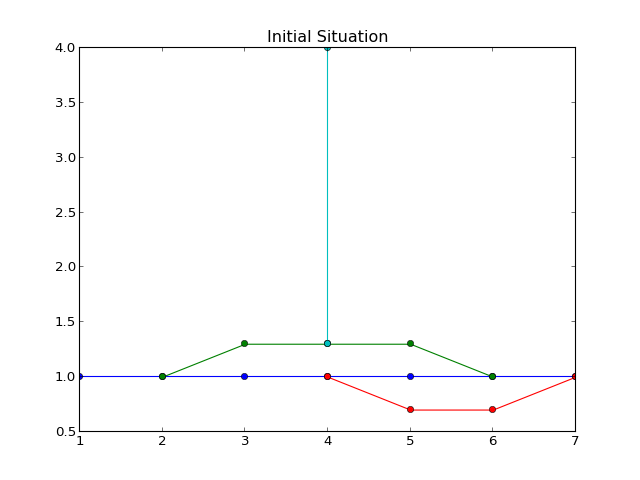
\includegraphics[scale=0.48]{comb-1.png}
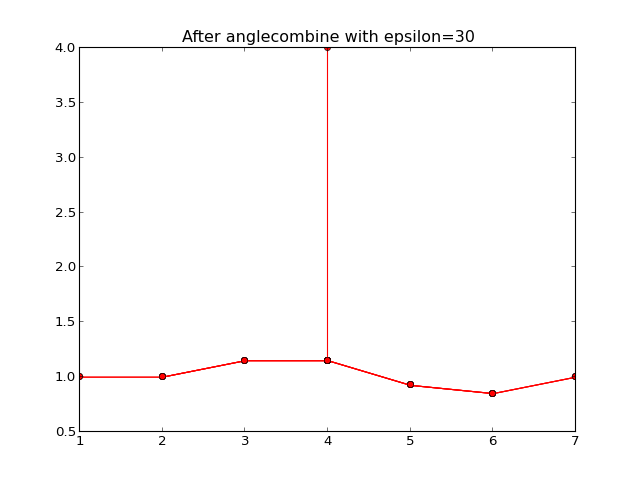
\includegraphics[scale=0.48]{comb-2.png}

\section{Network Segmentation}
\subsection{Intersection/Endpoint Segmentation Algorithm}
Segments a network graph. Segments are defined by its bounds, which are
either endpoints or intersections.
\subsection{Continuous Intersection/Endpoint Segmentation Algorithm}
Like the previous algorithm, but tries to extend the current segment based
on the angle between the last point of the segment and its neighbors.
\newpage

\section{Line Simplification}
\subsection{Angle-based reduction}
Removes a point if the angle between a point and its two neighbors
is greater than a threshold value.\\
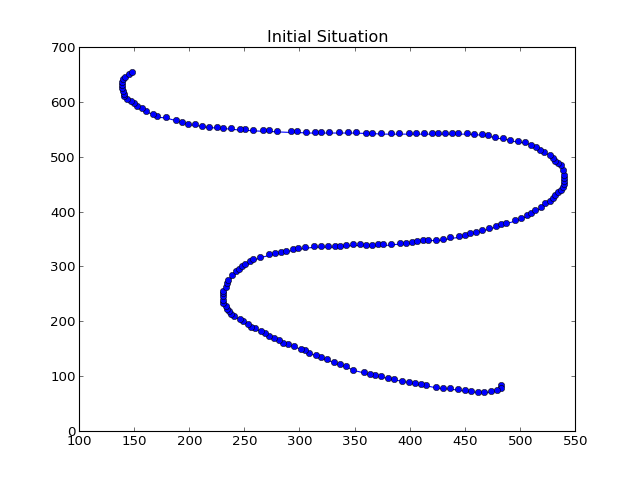
\includegraphics[scale=0.48]{simp-1.png}
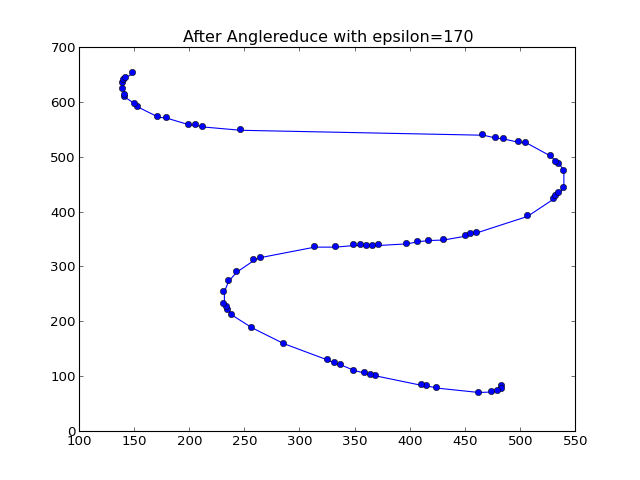
\includegraphics[scale=0.48]{simp-2.png}
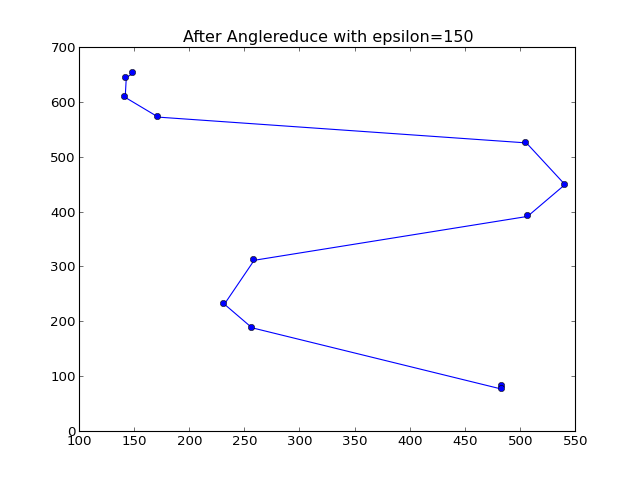
\includegraphics[scale=0.48]{simp-3.png}\\
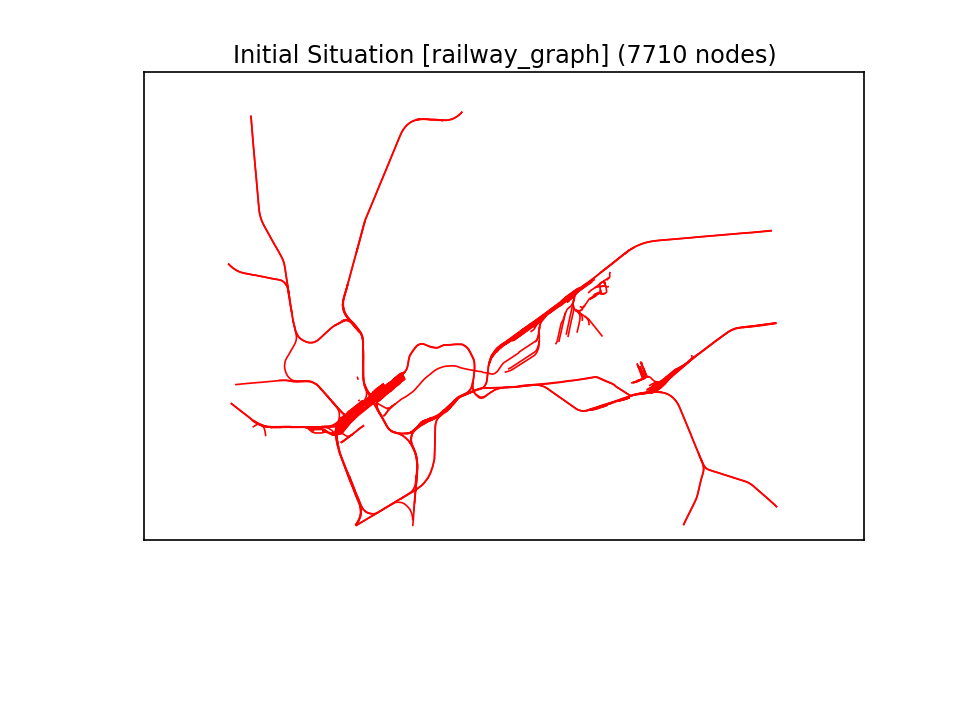
\includegraphics[scale=0.49]{anglered-1.png}
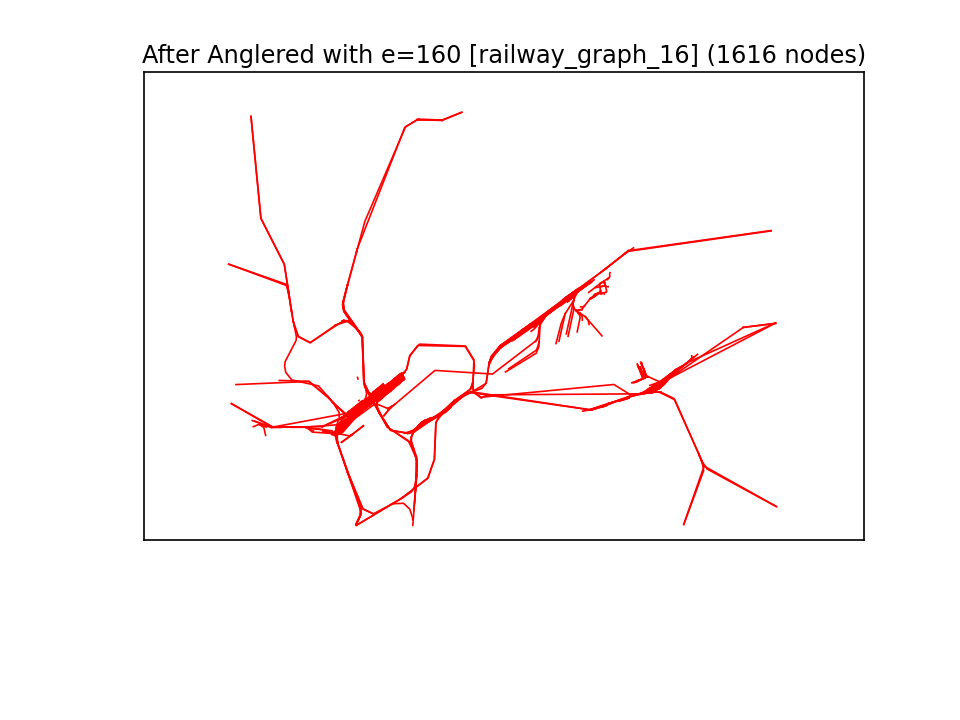
\includegraphics[scale=0.49]{anglered-2.png}

\subsection{Ramer-Douglas-Peucker Algorithm}
Based on maximum threshold distance between a point and the approximated
line segment.\\
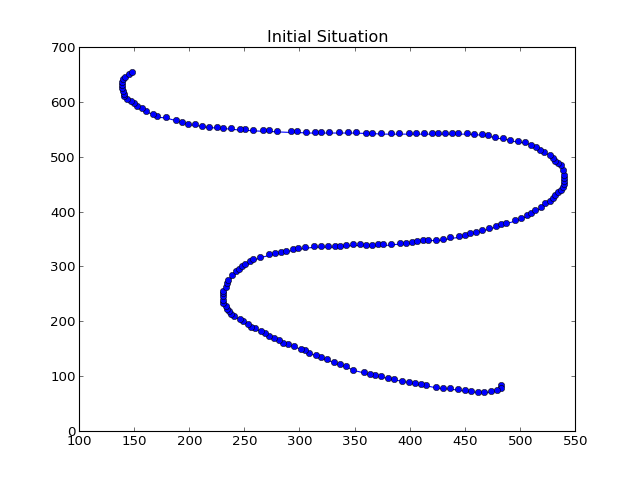
\includegraphics[scale=0.48]{simp-4.png}
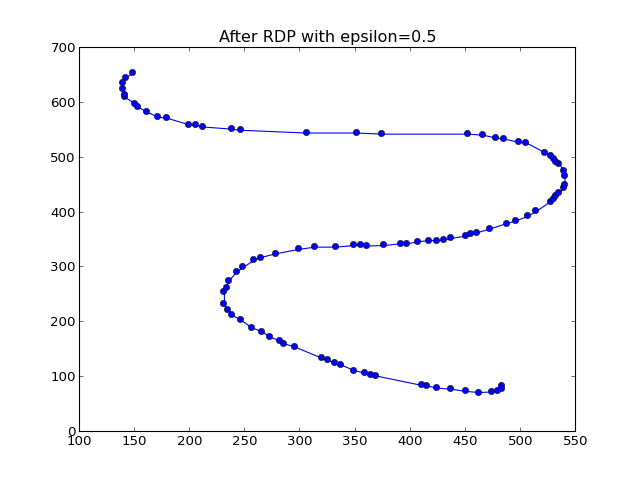
\includegraphics[scale=0.48]{simp-5.png}
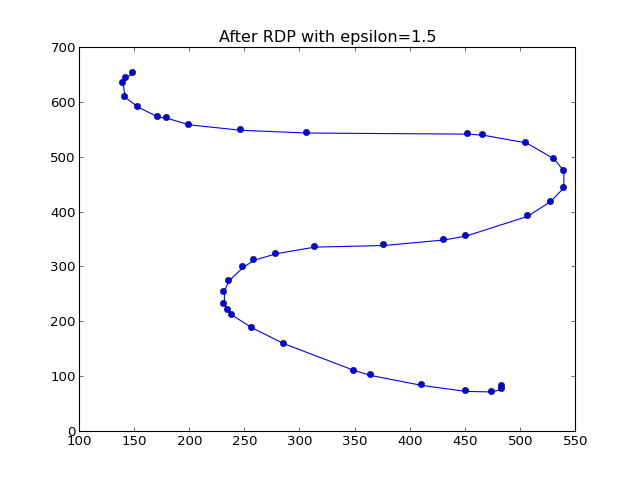
\includegraphics[scale=0.48]{simp-6.png}\\
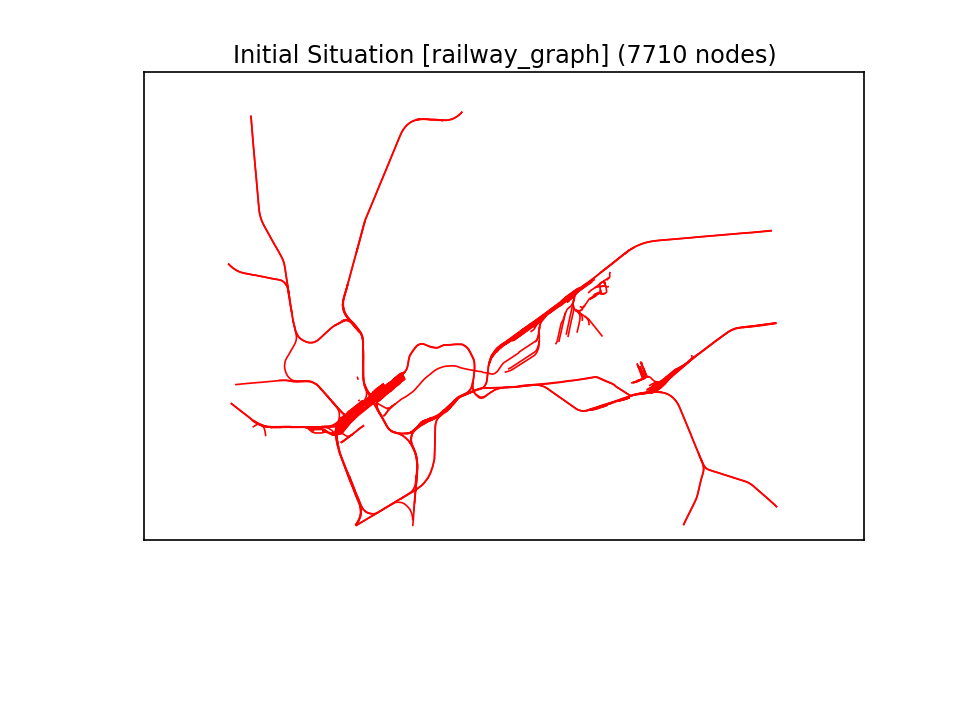
\includegraphics[scale=0.49]{rdprg-1.png}
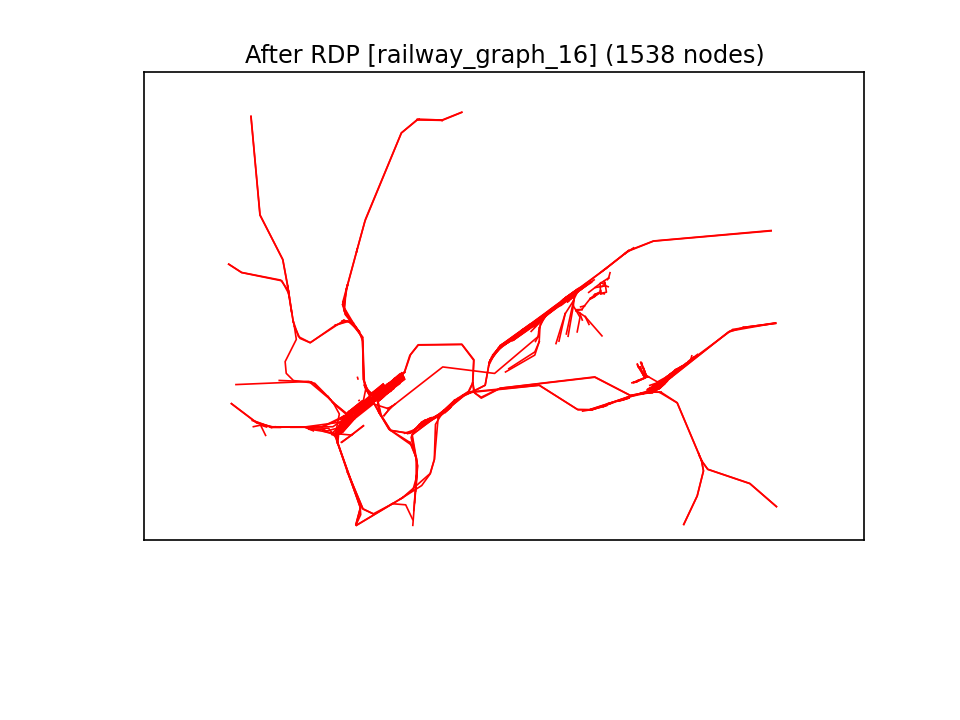
\includegraphics[scale=0.49]{rdprg-2.png}

\subsection{Rating-based Algorithms}
Based on an enriched Railway-Graph -- currently with the number of routes
involved, "notable" points planned.\\\\
Resulting algorithms will select the
\begin{itemize}
\item highest rated \(n\) nodes
\item nodes with a rating exceeding a threshold \(t\)
\end{itemize}
for inclusion.
\(n\) and \(t\) depend on the zoom  level.
Mostly suitable for higher zoom levels.

\section{Alternative Railway-Graph}
We build a alternative Railway Graph based on \texttt{Stations.txt} and
\texttt{sgrv.csv} yielding a drastically reduced RG suitable for higher zoom
levels.

\section{Notes}
\begin{itemize}
    \item Algorithms work on mercator projection
\end{itemize}

\section{Metric}
We have (at least) the following data available (per segment)

\begin{itemize}
\item length
\item removed nodes
\item overall points
\end{itemize}

From those we will derive the following metrics:

\begin{itemize}
\item distance to target amount of nodes per area (depending on zoomlevel)
\item importance of removed points (according to above rating)
\item distance of removed nodes to simplified segment
\end{itemize}

\section{Documentation}
Online documentation is available at \url{http://algolab.0x0b.de}.\\\\
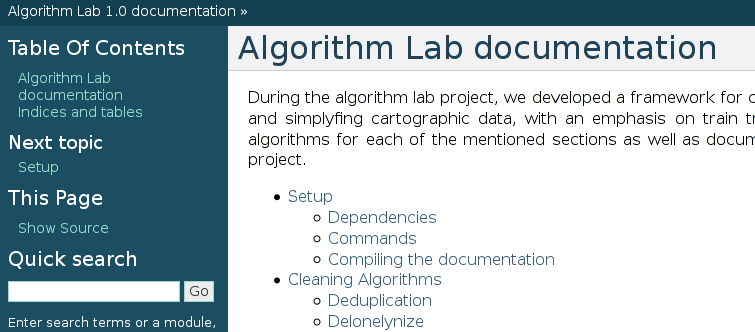
\includegraphics[scale=0.5]{doc.png}

\section{Test coverage}
\begin{verbatim}
Name                                Stmts   Miss  Cover
-------------------------------------------------------
algolab/__init__                        0      0   100%
algolab/combine/__init__                2      0   100%
algolab/combine/anglecombine           32      1    97%
algolab/data                           39      0   100%
algolab/db                            102     20    80%
algolab/segment/__init__               16      4    75%
algolab/segment/essegmenter            85     39    54%
algolab/simplify/__init__              23     13    43%
algolab/simplify/anglered              20      2    90%
algolab/simplify/rdp                   18      0   100%
algolab/simplify/rminner                2      0   100%
algolab/tests/__init__                  0      0   100%
algolab/tests/test_all                 51      0   100%
algolab/tests/test_combine             25      0   100%
algolab/tests/test_db                  72      0   100%
algolab/tests/test_segment             57      3    95%
algolab/tests/test_simplification      51      0   100%
algolab/util                           95     29    69%
-------------------------------------------------------
TOTAL                                 690    111    84%
\end{verbatim}

\section{Open Questions}
\begin{itemize}
    \item Node distance: Great-circle distance? Euclidean distance on mercator projection?
    \item Command Line Interface user-friendly?
    \item Selection of points representing stations?
    \item layout of \texttt{Stations.txt} and \texttt{sgrv.csv}
\end{itemize}

\newpage
\section{Appendix}
Ramer-Douglas-Peucker visualization:\\
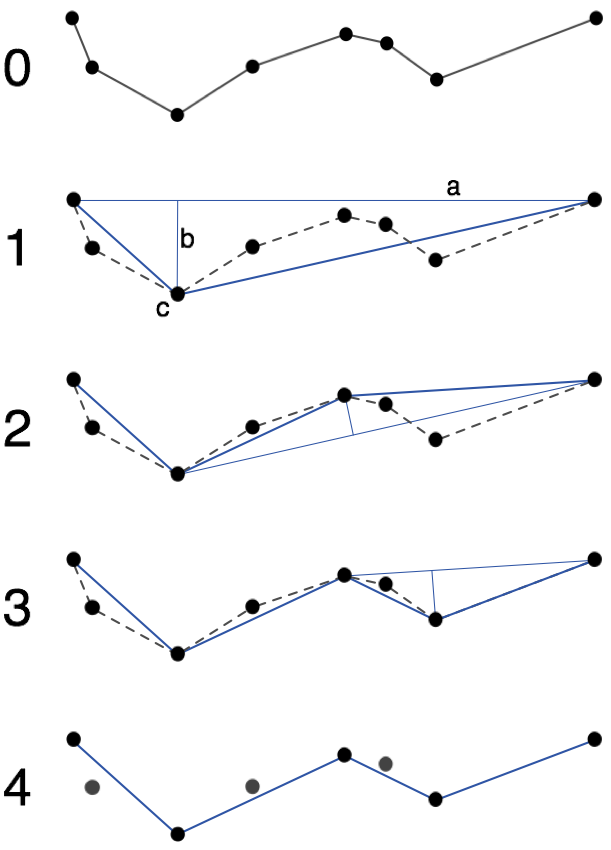
\includegraphics[scale=0.6]{rdp.png}
\end{document}
